\section{State Minimization (Book)}

It is important to be able to \textit{minimize the number of states} of a given deterministic finite automaton, that is, to determine an equivalent deterministic finite automaton that has as few states as possible. We shall next develop the necessary concepts and results that lead to such a \textit{state minimization algorithm}.

\begin{figure}[h!]
  \centering
  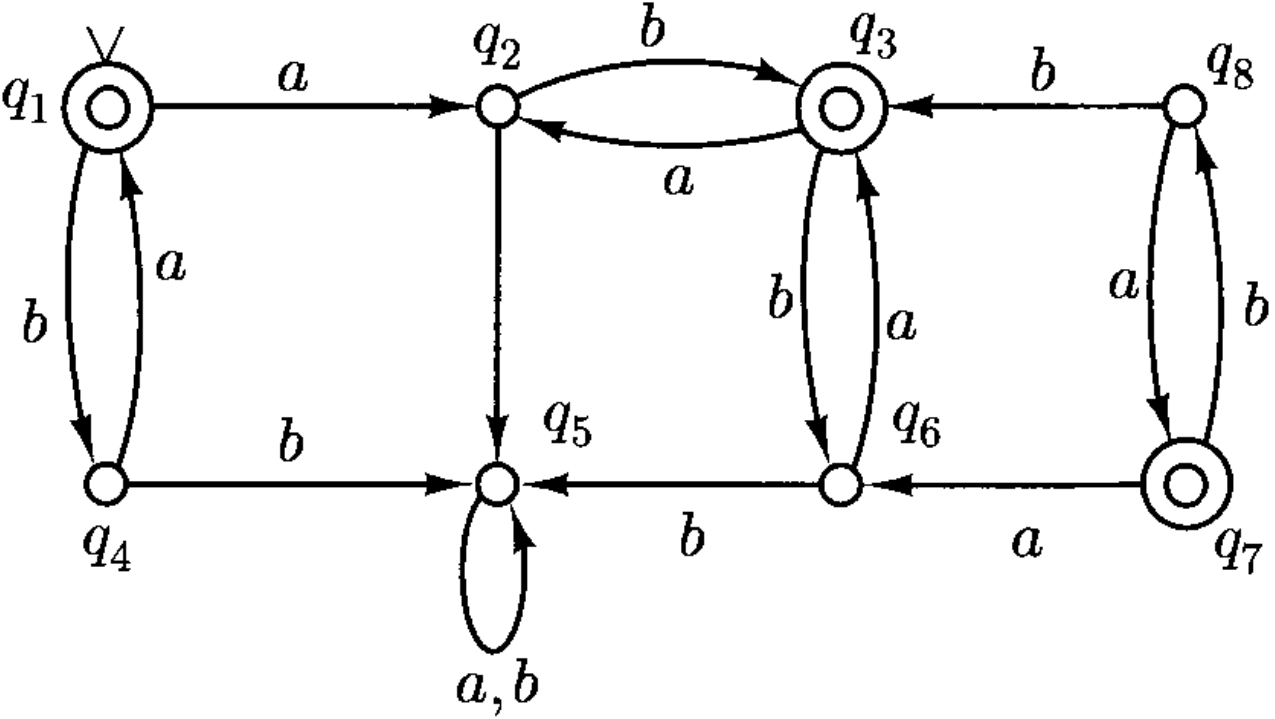
\includegraphics[width=.4\textwidth]{img/Fig2.19.png}
  \caption{}
\end{figure}

Given a deterministic finite automaton, there may be an easy way to get rid of several states. Let us take, for example, the deterministic automaton in Figure 16, accepting the language $L = (ab \cup ba)^*$. 

Consider state $q_7$. It should be clear that this state is \textit{unreachable}, because there is no path from the start state to it in the state diagram of the automaton. This is the simplest kind of optimization one can do on any deterministic finite automaton:\textit{ Remove all unreachable states and all transitions in and out of them}. In fact, this optimization was implicit in our conversion of a nondeterministic finite automaton to its equivalent deterministic one: We omitted from consideration all states that are not reachable from the start state of the resulting automaton.

Identifying the reachable states is easy to do in polynomial time, because the set of reachable states can be defined as the closure of $\{s\}$ under the relation $\left\{ (p, q)\ |\ \delta(p, a) = q \textnormal{ for some } a \in \Sigma \right\}$. Therefore,the set of all reachable states can be computed by this simple algorithm.

\begin{algorithm}
  \begin{algorithmic}
    \State $R$ := $\{s\}$
    \While{there is a state $p \in R$ and $a \in \Sigma$ such that $\delta(p, a) \notin R$}
      \State add $\delta(p, a)$ to $R$
    \EndWhile
\end{algorithmic}
\end{algorithm}

\begin{figure}[h!]
  \centering
  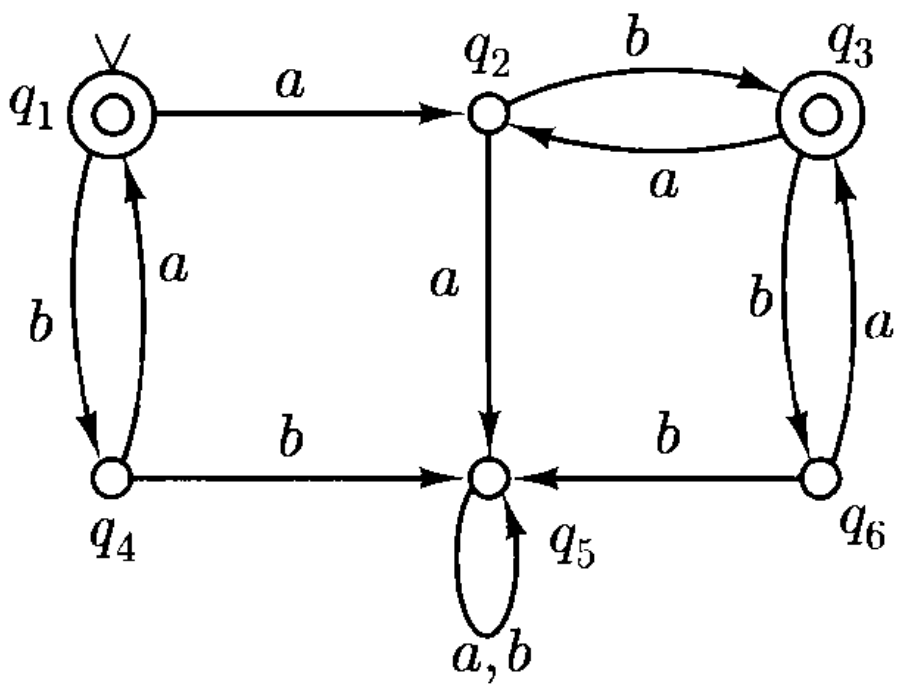
\includegraphics[width=.3\textwidth]{img/Fig2.20.png}
  \caption{}
\end{figure}

However, the remaining automaton after the deletion of unreachable states (Figure 17) still has more states than are really needed, this time for subtler reasons. For example, states $q_4$ and $q_6$ are equivalent, and therefore they \textit{can be merged into one state}. What does this mean, exactly? Intuitively, the reason we call these states equivalent is that, from \textit{either state, precisely the same strings lead the automaton to acceptance}.

\begin{definition}{}
  Let $L \subseteq \Sigma^*$ be a language, and let $x, y \in \Sigma^*$. We say that $x$ and $y$ are \textbf{equivalent with respect to $L$}, denoted $x \approx_L y$, if for all $z \in \Sigma^*$, the following is true: $xz \in L$ if and only if $yz \in L$. Notice that $\approx_L$ is an equivalence relation. 
\end{definition}

That is, $x \approx_L y$ if either both strings belong to $L$ or neither is in $L$; and moreover, appending any fixed string to both $x$ and $y$ results in two strings that are either both in $L$ or both not in $L$. (In other words, if $x \approx_L y$, then either $x, y \in L$ or $x, y \notin L$ (why?). In addition, if $x \approx_L y$, then appending the same string $z$ to both of them results in two strings that are either both in $L$ or both not in $L$.)

\begin{example}{}
  If $x$ is a string, and when $L$ is understood by context, we denote by $\left[ x \right]$ the equivalence class with respect to $L$ to which $x$ belongs. For example, for the language $L = (ab \cup ba)^*$ accepted by the automaton in Figure 17, it is not hard to see that $\approx_L$ has four equivalence classes:
  \begin{itemize}
    \item $\left[ e \right] = L$
    \item $\left[ a \right] = La$
    \item $\left[ b \right] = Lb$
    \item $\left[ aa \right] = L(aa \cup bb) \Sigma^*$
  \end{itemize}
  In (1), for any string $x \in L$, including $x = e$, the $z$'s that make $xz \in L$ are precisely the members of $L$. In (2), any $x \in La$ needs a $z$ of the form $bL$ in order for $xz$ to be in $L$. Similarly, for (3) the $z$'s are of the form $aL$. Finally, in (4) there is no $z$ that can restore to $L$ a string with a prefix in $L(aa \cup bb)$. In other words, all strings in set (1) have the same fate with respect to inclusion in $L$; and the same for (2), (3), and (4). Finally, it is easy to see that these four classes exhaust all of $\Sigma^*$. Hence these are the equivalence classes of $\approx_L$.
\end{example}

Notice that $\approx_L$ relates strings in terms of a language, not in terms of an automaton. Automata provide another, somewhat less fundamental, relation, described next.

\begin{definition}{}
  Let $M = (K, \Sigma, \delta, s, F)$ be a deterministic finite automaton. We say that two strings $x, y \in \Sigma^*$ are \textbf{equivalent with respect} to $M$, denoted $x \sim_M y$, if, intuitively, they both drive $M$ from $s$ to the same state. Formally, $x \sim_M y$ if there is a state $q$ such that $(s, x) \vdash_M^* (q, e)$ and $(s, y) \vdash_M^* (q, e)$.

  \quad Again, $\sim_M$ is an equivalence relation. Its equivalence classes can be identified by the states of $M$ -more precisely, with \textbf{\textit{those states that are reachable from $s$ and therefore have at least one string in the corresponding equivalence class}}. We denote the equivalence class corresponding to state $q$ of $M$ as $E_q$.
\end{definition}

\setcounter{example}{9}
\begin{example}{ continued}
  For example, for the automaton $M$ in Figure 17, the equivalence classes of $\sim_M$ are these (where $L = (ab \cup ba)^*$ is the language accepted by $M$)
  \begin{enumerate}
    \item $E_{q_1} = (ba)^*$ (by reading, $q_1$ is reachable from $s$)
    \item $E_{q_2} = La \cup a$ (by reading, $q_2$ is reachable from $s$)
    \item $E_{q_3} = abL$ (by reading, $q_3$ is reachable from $s$ and so on)
    \item $E_{q_4} = b (ab)^*$
    \item $E_{q_5} = L(bb \cup aa)\Sigma^*$
    \item $E_{q_6} = abLb$
  \end{enumerate}
  Again, they form a partition of $\Sigma^*$.
\end{example}

These two important equivalence relations, one associated with the language, the other with the automaton, are related as follows:

\begin{theorem}{}
  For any deterministic finite automaton $M = \left( K, \Sigma, \delta, s, F \right)$ and any strings $x, y \in \Sigma^*$, if $x \sim_M y$, then $x \approx_{L(M)} y$.   
\end{theorem}

\begin{proof}
  For any string $x \in \Sigma^*$, let $q(x) \in K$ be the unique state such that $(s, x) \vdash_M^* (q(x), e)$. Notice that, for any $x,z \in \Sigma^*$, $xz \in L(M)$ if and only if $(q(x), z) \vdash_M^* (f,e)$ for some $f \in F$. Now, if $x \sim_M y$ then, by the definition of $\sim_M$, $q(x) = q(y)$, and thus $x \sim_M y$ implies that the following holds:
  \begin{equation*}
    xz \in L(M) \textnormal{ if and only if } yz \in L(M) \textnormal{ for all } z \in \Sigma^*
  \end{equation*}
  which is the same as $x \approx_{L(M)} y$.
\end{proof}

A very suggestive way of expressing Theorem 5 is to say that $\sim_M$ is
a \textbf{refinement} of $\approx_{L(M)}$. In general, we say that an equivalence relation $\sim$ is a refinement of another $\approx$ if for all $x, y$ $x \sim y$ implies $x \approx y$. If $\sim$ is a refinement of $\approx$, then each equivalence class with respect to $\approx$ is contained in some equivalence class of $\approx$; that is, each equivalence class of $\approx$ is the union of one or more equivalence classes of $\sim$.

\setcounter{example}{9}
\begin{example}{ continued}
  For an example that is more to the point, the equivalence classes of $\sim_M$ for the automaton $M$ in Figure 17 ``refine'' in this sense the equivalence classes of $\approx_{L(M)}$, exactly as predicted by Theorem 5. For example, classes $E_{q_5}$ and $\left[aa\right]$ coincide, while classes $E_{q_1}$ and $E_{q_3}$ are both subsets of $\left[ e \right]$.
\end{example}

Theorem 5 implies something very important about $M$ and any other automaton $M'$ accepting the same language $L(M)$: Its number of states must be at least as large as the number of equivalence classes of $L(M)$ under $\approx_{L(M)}$. Thus, the number of equivalence classes of $\approx_{L(M)}$ gives a lower bound on the number of states of an automaton $M'$ that accepts $L(M)$.

\begin{theorem}{: The Myhill-Nerode Theorem}
  Let $L \subseteq \Sigma^*$ be a regular language. Then there is a deterministic finite automaton $M = (K, \Sigma, \delta, s, F)$ with precisely as many states as there are equivalence classes in $\approx_L$ that accepts $L$. In other words, $L = L(M)$and $|K|$ is the number of equivalence classes of $\approx_L$.
\end{theorem}

\begin{multicols}{2}
\setlength{\columnsep}{1.5cm}
\setlength{\columnseprule}{0.2pt}
\begin{proof}
  As before, we denote the equivalence class of string $x \in \Sigma^*$ in the equivalence relation $\approx_L$ by $\left[x\right]$. Given $L$, we shall construct a deterministic finite automaton (the \textbf{standard automaton} for $L$) $M = (K, \Sigma, \delta, s, F)$ such that $L = L(M)$. $M$ is defined as follows:
  \begin{itemize}
    \item $K = \left\{ \left[x\right] : x \in \Sigma^*\right\}$, the set of equivalence classes under $\approx_L$.
    \item $s = \left[e\right]$, the equivalence class of $e$ under $\approx_L$.
    \item $F = \left\{ \left[ x \right] : x \in L \right\}$
    \item Finally, for any $\left[ x \right] \in K$ and any $a \in \Sigma$, define $\delta(\left[ x \right], a) = \left[ xa \right]$.
  \end{itemize}
  How do we know that the set $K$ is finite, that is, that $\approx_L$ has finitely many equivalent classes? $L$ is regular, and so it is surely accepted by some deterministic finite automaton $M'$. By the previous theorem, $\sim_{M'}$ is a refinement of $\approx_L$, and so there are fewer equivalence classes in $L$ than there are equivalence classes of $\sim_{M'}$ -that is to say, states of $M'$. Hence $K$ is a finite set. We also have to argue that $\delta$ is \textit{well defined}, that is, $\delta(\left[ x \right], a) = \left[ xa \right]$ is independent of the string $x \in \left[ x \right]$. But this is easy to see, because $x \approx_L x'$ if and only if $xa \approx_L x'a$.

  We next show that $L = L(M)$. First we show that for all $x, y \in \Sigma^*$, we have
  \begin{equation}
    \left( \left[ x \right], y \right) \vdash_M^* \left( \left[ xy \right], e \right)
  \end{equation}
  This is established by induction on $|y|$. It is trivial when $y = e$, and, if it holds for all $y$'s of length up to $n$ and $y = y'a$, then by induction $\left( \left[ x \right], y'a \right) \vdash_M^* \left( \left[ xy' \right], a \right) \vdash_M^* \left( \left[ xy \right], e \right)$.
  
  Now (1) completes the proof: For all $x \in \Sigma^*$, we have that $x \in L(M)$ if and only if $\left( \left[ e \right], x \right) \vdash *\left( q, e \right)$ for some $q \in F$, which is by (1) the same as saying $\left[ x \right] \in F$, or, by the deinition of $F$, $\left[ x \in L \right]$.
\end{proof}
\end{multicols}

\setcounter{example}{9}
\begin{example}{ continued}
  The standard automaton corresponding to the language $L = (ab \cup ba)^*$ accepted by the six-state deterministic finite automaton in Figure 17 is shown in Figure 18. It has \textit{four} states. Naturally, it is the smallest deterministic finite automaton that accepts this language.
\end{example}

\begin{figure}[h]
  \centering
  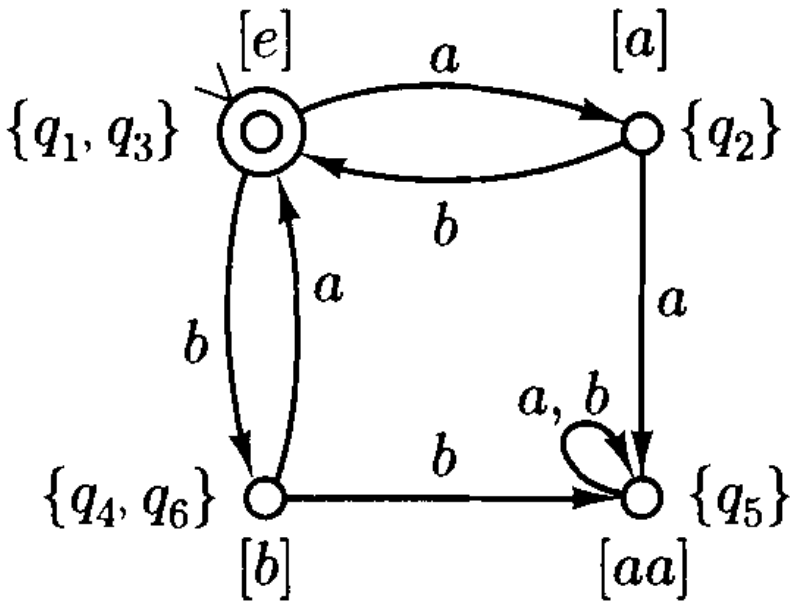
\includegraphics[width=.5\textwidth]{img/Fig2.21.png}
  \caption{}
\end{figure}

Incidentally, Theorems 6 immediately imply the following characterization of regular languages, sometimes itself called the \textit{Myhill-Nerode Theorem}:

\begin{formula}{Corollary}
  \textit{A language $L$ is regular if and only if $\approx_L$ has finitely many equivalence classes.}
\end{formula}

\begin{proof}
  If $L$ is regular, then $L = L(M)$ for some deterministic finite automaton $M$, and $M$ has at least as many states as $\approx_L$ has equivalence classes. Hence there are finitely many equivalence classes in $\approx_L$.

  \quad Conversely, if $\approx_L$ has finitely many equivalence classes, then the standard deterministic finite automaton $M_L$ (recall the proof of Theorem 6) accepts $L$.
\end{proof}

The corollary can be used to show that a language is not regular (show that it has infinitely many equivalence classes).

\begin{example}{}
  The corollary just proved is an interesting alternative way of specifying what it means for a language $L$ to be regular. Furthermore, it provides another useful way for proving that a language is not regular -besides the Pumping Theorem.

  For example, here is an alternative proof that $L = \{a^nb^n : n \geq 1\}$ is not regular: No two strings $a^i$ and $a^j$, with $i \neq j$, are equivalent under $\approx_L$, simply because there is a string (namely, $b^i$) which, when affixed $a^i$ gives a string in $L$, but when affixed to $a^j$ produces a string not in $L$. Hence $\approx_L$ has infinitely
  many equivalence classes $\left[ e \right], \left[ a \right], \left[ aa \right], \left[ aaa \right], ...$, and hence by the corollary $L$ is
  not regular.
\end{example}

\begin{multicols}{2}
\setlength{\columnsep}{1.5cm}
\setlength{\columnseprule}{0.2pt}
  For any regular language $L$ the automaton constructed in the proof of Theorem 6 is the deterministic automaton with the \textit{fewest states} that accepts $L$. Unfortunately, this automaton is defined in terms of the equivalence classes of $\approx_L$, and it is not clear how these equivalence classes can be identified for any given regular language $L$. We shall next develop an \textit{algorithm} for constructing this minimal automaton, starting from \textit{any deterministic finite automaton $M$} such that $L = L(M)$.
  
  Let $M = (K, \Sigma, \delta, s, F)$ be a deterministic finite automaton. Define a relation $A_M \subseteq K \times \Sigma^*$, as follows: $(q, w) \in A_M$ if and only if $(q, w) \vdash_M^* (f, e)$ for some $f \in F$; that is, $(q, w) \in A_M$ means that $w$ drives $M$ from $q$ to an accepting state. 
  
  Let us call two states $q, p \in K$ \textbf{equivalent}, denoted $q \equiv p$, if the following holds for all $z \in \Sigma^*$: $(q, z) \in A_M$ if and only if $(p, z) \in A_M$. Thus, if two states are equivalent, then the corresponding equivalence classes of $\sim_M$ are subsets of the same equivalence class of $\approx_L$.
  
  In other words, the equivalence classes of $\equiv$ are precisely those sets of states of $M$ that must be clumped together in order to obtain the standard automaton of $L(M)$.
  
  We shall develop an algorithm for computing the equivalence classes of $\equiv$. Our algorithm will compute $\equiv$ as the \textit{limit} of a sequence of equivalence relations $\equiv_0, \equiv_1, \equiv_2, ...$, defined next. For two states $q, p \in K$, $q \equiv_n p$ if the following is true: $(q, z) \in A_M$ if and only if $(p, z) \in A_M$ for all strings $z$ such that $|z| \leq n$. In other words, $\equiv_n$ is a \textit{coarser} equivalence relation than $\equiv$, only requiring that states $q$ and $p$ behave the same with respect to acceptance when driven by strings of \textit{length up to $n$}.

  Obviously, each equivalence relation in $\equiv_0, \equiv_1, \equiv_2, ...$ is a refinement of the previous one. Also, $q \equiv_0 p$ holds if $q$ and $p$ are either both accepting, or both non-accepting. That is, there are precisely two equivalence classes of $\equiv_0$: $F$ and $K - F$ (assuming they are both nonempty). It remains to show how $\equiv_{n+1}$ depends on $\equiv_n$. Here is how:
\end{multicols}

\begin{formula}{Lemma 1}
  \textit{For any two states $q, p \in K$ and any integer $n \geq 1$, $q \equiv_n p$ if and only if}
  \begin{enumerate}[label=\alph*)]
    \item $q \equiv_{n-1} p$, and 
    \item for all $a \in \Sigma$, $\delta(q, a) \equiv_{n-1} \delta(p, a)$.
  \end{enumerate}

  [Basically, there should be a string $z$ such that $(q, z) \in A_M$ and $(p, z) \in A_M$. To be inside $A_M$, there should be strings $w, w'$ such that $(q, w) \vdash_M^* (f,e)$ and $(p, w') \vdash_M^* (f,e)$. So if $q \equiv_{n-1} p$, and there is transition from $q$ and $p$, they can reach the step $n$.]
\end{formula}

\begin{proof}
  By definition of $\equiv_n$, $q \equiv_n p$ if and only if $q \equiv_{n-1} p$, and furthermore any string $w = av$ of length precisely $n$ drives either both $q$ and $p$ to acceptance, or both to nonacceptance. However, the second condition is the same as saying that $\delta(q, a) \equiv_{n-1} \delta(p, a)$ for any $a \in \Sigma$.
\end{proof}

Lemma 1 suggests that we can compute $\equiv$, and from this the standard
automaton for $L$, by the following algorithm:

\begin{algorithm}
  \begin{algorithmic}
    \State \texttt{Initially the equivalence classes of $\equiv_0$ are $F$ and $K - F$}
    \While{$\equiv_n\ \neq\ \equiv_{n-1}$} 
      \Comment{Repeat for $n := 1,2, ...$ until $\equiv_n$ is the same as $\equiv_{n-1}$.}
      \State \texttt{Compute the equivalence classes of $\equiv_n$ from those $\equiv_{n-1}$}
      \State (for each $a \in \Sigma$, and equivalence class $[q]$, compute $\{ \delta(q', a)\ |\ q' \in [q] \}$, and split the equivalence classes that intersect with this set)
    \EndWhile
\end{algorithmic}
\end{algorithm}

Each iteration can be carried out by applying Lemma 1: For each pair of states of $M$, we test whether the conditions of the lemma hold, and if so we put the two states in the same equivalence class of $\equiv_n$.

But how do we know that this is an algorithm, that the iteration will eventually terminate? The answer is simple: For each iteration at which the termination condition is not satisfied, ($\equiv_n\ \neq\ \equiv_{n-1}$), $\equiv_n$ is a \textit{proper refinement} of $\equiv_{n-1}$, and thus has at least one more equivalence class than $\equiv_{n-1}$. Since the number of equivalence classes cannot become more than the number of states of $M$, the algorithm will terminate after at most $|K| - 1$ iterations.

When the algorithm terminates, say at the $n$th iteration and having computed $\equiv_{n} = \equiv_{n-1}$, then the lemma implies that $\equiv_{n} = \equiv_{n+1} = \equiv_{n+2} = \equiv_{n+3} = ...$. Hence the relation computed is precisely $\equiv$.

\begin{figure}[ht]
  \centering
  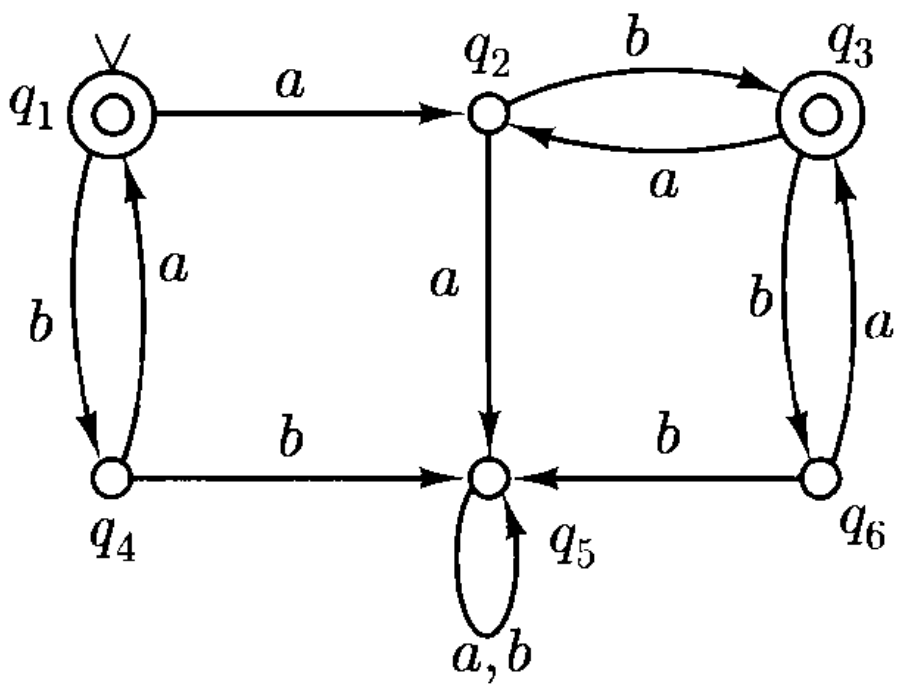
\includegraphics[width=.25\textwidth]{./img/Fig2.20.png}
  \caption{}
\end{figure}

\begin{example}{}
  Let us apply the state minimization algorithm to the deterministic finite automaton $M$ in Figure 19 (same with 17). At the various iterations we shall have these equivalence classes of the corresponding $\equiv_i$:
  \begin{itemize}
    \item Initially, the equivalence classes of $\equiv_{0}$ are $\left\{ q_1, q_3 \right\}$ and $\left\{ q_2, q_4, q_5, q_6 \right\}$.
    \item After the first iteration, the classes of $\equiv_{1}$ are $\left\{ q_1, q_3 \right\}$, $\left\{ q_2 \right\}$, $\left\{ q_4, q_6 \right\}$, and $\left\{ q_5 \right\}$. The splitting happened because $\delta(q_2, b) \not\equiv_{0} \delta(q_4, b), \delta(q_5,b)$, and $\delta(q_4, a) \not\equiv_{0} \delta(q_5,a)$.
    \item After the second iteration, there is no further splitting of classes. The algorithm thus terminates, and the minimum-state automaton is shown in Figure 20. As expected, it is isomorphic with the standard automaton shown in Figure 18.
  \end{itemize}
\end{example}

\begin{figure}[ht]
  \centering
  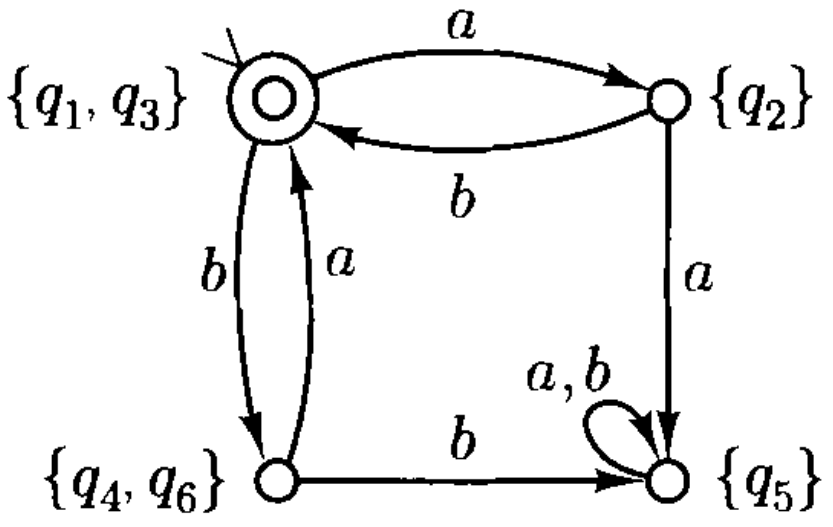
\includegraphics[width=.25\textwidth]{./img/fig2-22.png}
  \caption{}
\end{figure}
